% Options for packages loaded elsewhere
\PassOptionsToPackage{unicode}{hyperref}
\PassOptionsToPackage{hyphens}{url}
\PassOptionsToPackage{dvipsnames,svgnames*,x11names*}{xcolor}
%
\documentclass[
]{article}
\usepackage{amsmath,amssymb}
\usepackage{lmodern}
\usepackage{ifxetex,ifluatex}
\ifnum 0\ifxetex 1\fi\ifluatex 1\fi=0 % if pdftex
  \usepackage[T1]{fontenc}
  \usepackage[utf8]{inputenc}
  \usepackage{textcomp} % provide euro and other symbols
\else % if luatex or xetex
  \usepackage{unicode-math}
  \defaultfontfeatures{Scale=MatchLowercase}
  \defaultfontfeatures[\rmfamily]{Ligatures=TeX,Scale=1}
\fi
% Use upquote if available, for straight quotes in verbatim environments
\IfFileExists{upquote.sty}{\usepackage{upquote}}{}
\IfFileExists{microtype.sty}{% use microtype if available
  \usepackage[]{microtype}
  \UseMicrotypeSet[protrusion]{basicmath} % disable protrusion for tt fonts
}{}
\makeatletter
\@ifundefined{KOMAClassName}{% if non-KOMA class
  \IfFileExists{parskip.sty}{%
    \usepackage{parskip}
  }{% else
    \setlength{\parindent}{0pt}
    \setlength{\parskip}{6pt plus 2pt minus 1pt}}
}{% if KOMA class
  \KOMAoptions{parskip=half}}
\makeatother
\usepackage{xcolor}
\IfFileExists{xurl.sty}{\usepackage{xurl}}{} % add URL line breaks if available
\IfFileExists{bookmark.sty}{\usepackage{bookmark}}{\usepackage{hyperref}}
\hypersetup{
  pdftitle={Second Paper},
  pdfauthor={Ordinary Leading Students},
  colorlinks=true,
  linkcolor=Maroon,
  filecolor=Maroon,
  citecolor=Blue,
  urlcolor=blue,
  pdfcreator={LaTeX via pandoc}}
\urlstyle{same} % disable monospaced font for URLs
\usepackage[margin=1in]{geometry}
\usepackage{color}
\usepackage{fancyvrb}
\newcommand{\VerbBar}{|}
\newcommand{\VERB}{\Verb[commandchars=\\\{\}]}
\DefineVerbatimEnvironment{Highlighting}{Verbatim}{commandchars=\\\{\}}
% Add ',fontsize=\small' for more characters per line
\usepackage{framed}
\definecolor{shadecolor}{RGB}{248,248,248}
\newenvironment{Shaded}{\begin{snugshade}}{\end{snugshade}}
\newcommand{\AlertTok}[1]{\textcolor[rgb]{0.94,0.16,0.16}{#1}}
\newcommand{\AnnotationTok}[1]{\textcolor[rgb]{0.56,0.35,0.01}{\textbf{\textit{#1}}}}
\newcommand{\AttributeTok}[1]{\textcolor[rgb]{0.77,0.63,0.00}{#1}}
\newcommand{\BaseNTok}[1]{\textcolor[rgb]{0.00,0.00,0.81}{#1}}
\newcommand{\BuiltInTok}[1]{#1}
\newcommand{\CharTok}[1]{\textcolor[rgb]{0.31,0.60,0.02}{#1}}
\newcommand{\CommentTok}[1]{\textcolor[rgb]{0.56,0.35,0.01}{\textit{#1}}}
\newcommand{\CommentVarTok}[1]{\textcolor[rgb]{0.56,0.35,0.01}{\textbf{\textit{#1}}}}
\newcommand{\ConstantTok}[1]{\textcolor[rgb]{0.00,0.00,0.00}{#1}}
\newcommand{\ControlFlowTok}[1]{\textcolor[rgb]{0.13,0.29,0.53}{\textbf{#1}}}
\newcommand{\DataTypeTok}[1]{\textcolor[rgb]{0.13,0.29,0.53}{#1}}
\newcommand{\DecValTok}[1]{\textcolor[rgb]{0.00,0.00,0.81}{#1}}
\newcommand{\DocumentationTok}[1]{\textcolor[rgb]{0.56,0.35,0.01}{\textbf{\textit{#1}}}}
\newcommand{\ErrorTok}[1]{\textcolor[rgb]{0.64,0.00,0.00}{\textbf{#1}}}
\newcommand{\ExtensionTok}[1]{#1}
\newcommand{\FloatTok}[1]{\textcolor[rgb]{0.00,0.00,0.81}{#1}}
\newcommand{\FunctionTok}[1]{\textcolor[rgb]{0.00,0.00,0.00}{#1}}
\newcommand{\ImportTok}[1]{#1}
\newcommand{\InformationTok}[1]{\textcolor[rgb]{0.56,0.35,0.01}{\textbf{\textit{#1}}}}
\newcommand{\KeywordTok}[1]{\textcolor[rgb]{0.13,0.29,0.53}{\textbf{#1}}}
\newcommand{\NormalTok}[1]{#1}
\newcommand{\OperatorTok}[1]{\textcolor[rgb]{0.81,0.36,0.00}{\textbf{#1}}}
\newcommand{\OtherTok}[1]{\textcolor[rgb]{0.56,0.35,0.01}{#1}}
\newcommand{\PreprocessorTok}[1]{\textcolor[rgb]{0.56,0.35,0.01}{\textit{#1}}}
\newcommand{\RegionMarkerTok}[1]{#1}
\newcommand{\SpecialCharTok}[1]{\textcolor[rgb]{0.00,0.00,0.00}{#1}}
\newcommand{\SpecialStringTok}[1]{\textcolor[rgb]{0.31,0.60,0.02}{#1}}
\newcommand{\StringTok}[1]{\textcolor[rgb]{0.31,0.60,0.02}{#1}}
\newcommand{\VariableTok}[1]{\textcolor[rgb]{0.00,0.00,0.00}{#1}}
\newcommand{\VerbatimStringTok}[1]{\textcolor[rgb]{0.31,0.60,0.02}{#1}}
\newcommand{\WarningTok}[1]{\textcolor[rgb]{0.56,0.35,0.01}{\textbf{\textit{#1}}}}
\usepackage{graphicx}
\makeatletter
\def\maxwidth{\ifdim\Gin@nat@width>\linewidth\linewidth\else\Gin@nat@width\fi}
\def\maxheight{\ifdim\Gin@nat@height>\textheight\textheight\else\Gin@nat@height\fi}
\makeatother
% Scale images if necessary, so that they will not overflow the page
% margins by default, and it is still possible to overwrite the defaults
% using explicit options in \includegraphics[width, height, ...]{}
\setkeys{Gin}{width=\maxwidth,height=\maxheight,keepaspectratio}
% Set default figure placement to htbp
\makeatletter
\def\fps@figure{htbp}
\makeatother
\setlength{\emergencystretch}{3em} % prevent overfull lines
\providecommand{\tightlist}{%
  \setlength{\itemsep}{0pt}\setlength{\parskip}{0pt}}
\setcounter{secnumdepth}{-\maxdimen} % remove section numbering
\usepackage{subfig}
\usepackage{bbm}
\ifluatex
  \usepackage{selnolig}  % disable illegal ligatures
\fi

\title{Second Paper}
\author{Ordinary Leading Students}
\date{6/02/2021}

\begin{document}
\maketitle

\begin{abstract}
In this paper we are going to perform a cluster analysis on a dataset used for a 
market basket analysis. Our goal is to find unknown subgroups in the dataset.

\end{abstract}

\section{Data}

We will now load and present our dataset (that can be retrieved at the
following
\href{https://www.kaggle.com/vjchoudhary7/customer-segmentation-tutorial-in-python}{link}).

\begin{Shaded}
\begin{Highlighting}[]
\CommentTok{\# Set the working directory and load the dataset}
\FunctionTok{setwd}\NormalTok{(}\FunctionTok{dirname}\NormalTok{(rstudioapi}\SpecialCharTok{::}\FunctionTok{getSourceEditorContext}\NormalTok{()}\SpecialCharTok{$}\NormalTok{path))}

\NormalTok{malldt}\OtherTok{\textless{}{-}} \FunctionTok{read\_csv}\NormalTok{(}\StringTok{"Mall\_Customers.csv"}\NormalTok{)}

\CommentTok{\# Summary of the dataset without the id column}
\FunctionTok{summary}\NormalTok{(malldt[}\SpecialCharTok{{-}}\DecValTok{1}\NormalTok{])}
\end{Highlighting}
\end{Shaded}

\begin{verbatim}
##     Gender               Age        Annual Income (k$) Spending Score (1-100)
##  Length:200         Min.   :18.00   Min.   : 15.00     Min.   : 1.00         
##  Class :character   1st Qu.:28.75   1st Qu.: 41.50     1st Qu.:34.75         
##  Mode  :character   Median :36.00   Median : 61.50     Median :50.00         
##                     Mean   :38.85   Mean   : 60.56     Mean   :50.20         
##                     3rd Qu.:49.00   3rd Qu.: 78.00     3rd Qu.:73.00         
##                     Max.   :70.00   Max.   :137.00     Max.   :99.00
\end{verbatim}

\section{Data Cleaning}

We removed the \textbf{CustomerID} variable and converted the
\textbf{Gender} one in factor.

\begin{Shaded}
\begin{Highlighting}[]
\NormalTok{malldt}\SpecialCharTok{$}\NormalTok{CustomerID }\OtherTok{\textless{}{-}} \ConstantTok{NULL}
\NormalTok{malldt}\SpecialCharTok{$}\NormalTok{Gender }\OtherTok{\textless{}{-}} \FunctionTok{as.factor}\NormalTok{(malldt}\SpecialCharTok{$}\NormalTok{Gender)}
\end{Highlighting}
\end{Shaded}

\newpage

\section{Data Visualization}

\begin{Shaded}
\begin{Highlighting}[]
\CommentTok{\# Gender Boxplots}

\FunctionTok{par}\NormalTok{(}\AttributeTok{mfrow=}\FunctionTok{c}\NormalTok{(}\DecValTok{1}\NormalTok{,}\DecValTok{2}\NormalTok{))}
\FunctionTok{boxplot}\NormalTok{(}\StringTok{\textasciigrave{}}\AttributeTok{Annual Income (k$)}\StringTok{\textasciigrave{}}\SpecialCharTok{\textasciitilde{}}\NormalTok{Gender,}\AttributeTok{data=}\NormalTok{malldt, }\AttributeTok{col=}\StringTok{"\#2D708EFF"}\NormalTok{)}
\FunctionTok{boxplot}\NormalTok{(}\StringTok{\textasciigrave{}}\AttributeTok{Spending Score (1{-}100)}\StringTok{\textasciigrave{}}\SpecialCharTok{\textasciitilde{}}\NormalTok{Gender,}\AttributeTok{data=}\NormalTok{malldt, }\AttributeTok{col=}\StringTok{"darkgoldenrod2"}\NormalTok{)}
\end{Highlighting}
\end{Shaded}

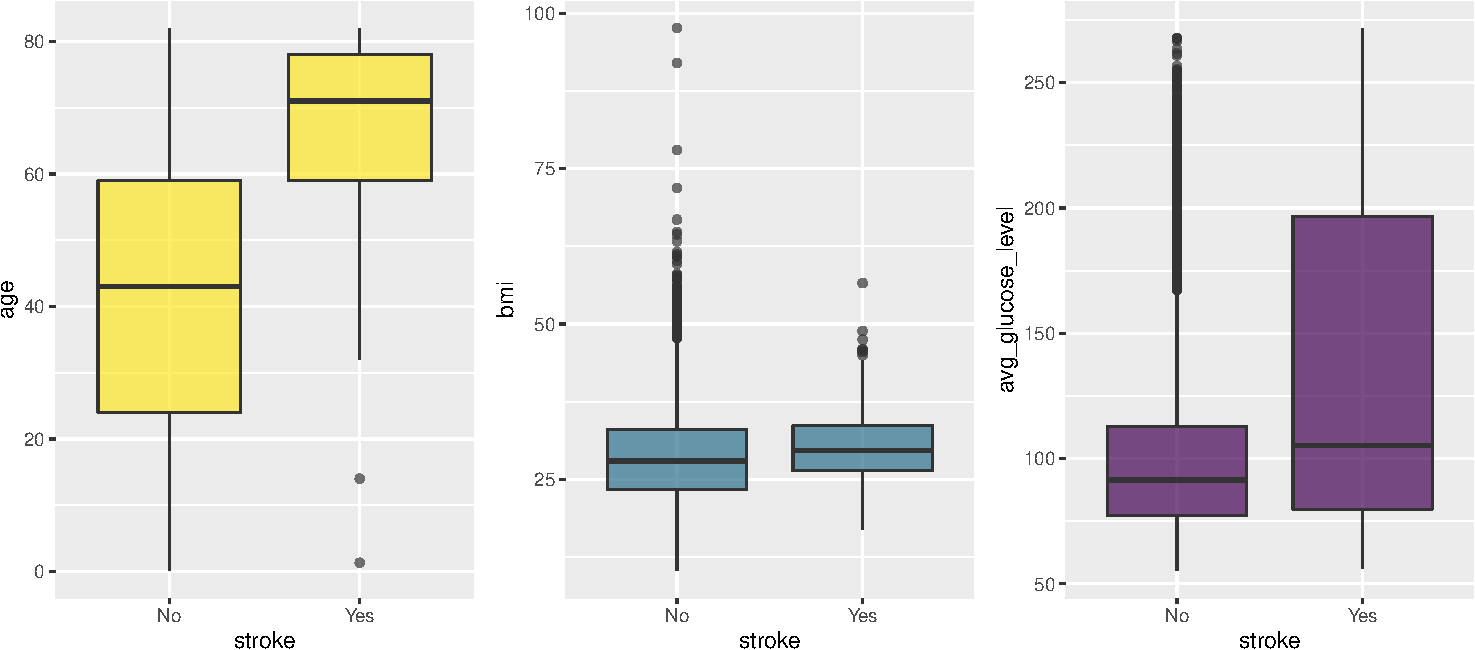
\includegraphics{report2_files/figure-latex/unnamed-chunk-4-1.pdf}

As we can see there are no meaningful differences between the genders
group.

\newpage

\begin{Shaded}
\begin{Highlighting}[]
\CommentTok{\# Age Boxplots}

\CommentTok{\# Create age groups}
\NormalTok{labs }\OtherTok{\textless{}{-}} \FunctionTok{c}\NormalTok{(}\FunctionTok{paste}\NormalTok{(}\FunctionTok{seq}\NormalTok{(}\DecValTok{15}\NormalTok{, }\DecValTok{70}\NormalTok{, }\AttributeTok{by =} \DecValTok{20}\NormalTok{), }\FunctionTok{seq}\NormalTok{(}\DecValTok{15} \SpecialCharTok{+} \DecValTok{20} \SpecialCharTok{{-}} \DecValTok{1}\NormalTok{, }\DecValTok{80}\NormalTok{, }\AttributeTok{by =} \DecValTok{20}\NormalTok{), }
                \AttributeTok{sep =} \StringTok{"{-}"}\NormalTok{))}

\NormalTok{malldt}\SpecialCharTok{$}\NormalTok{AgeGroup }\OtherTok{\textless{}{-}} \FunctionTok{cut}\NormalTok{(malldt}\SpecialCharTok{$}\NormalTok{Age, }\AttributeTok{breaks =} \FunctionTok{c}\NormalTok{(}\FunctionTok{seq}\NormalTok{(}\DecValTok{15}\NormalTok{, }\DecValTok{70}\NormalTok{, }\AttributeTok{by =} \DecValTok{20}\NormalTok{), }\ConstantTok{Inf}\NormalTok{), }
                       \AttributeTok{labels =}\NormalTok{ labs, }\AttributeTok{right =} \ConstantTok{FALSE}\NormalTok{)}

\FunctionTok{par}\NormalTok{(}\AttributeTok{mfrow=}\FunctionTok{c}\NormalTok{(}\DecValTok{1}\NormalTok{,}\DecValTok{2}\NormalTok{))}
\FunctionTok{boxplot}\NormalTok{(}\StringTok{\textasciigrave{}}\AttributeTok{Annual Income (k$)}\StringTok{\textasciigrave{}}\SpecialCharTok{\textasciitilde{}}\NormalTok{AgeGroup,}\AttributeTok{data=}\NormalTok{malldt, }\AttributeTok{col=}\StringTok{"\#FF99CC"}\NormalTok{)}
\FunctionTok{boxplot}\NormalTok{(}\StringTok{\textasciigrave{}}\AttributeTok{Spending Score (1{-}100)}\StringTok{\textasciigrave{}}\SpecialCharTok{\textasciitilde{}}\NormalTok{AgeGroup,}\AttributeTok{data=}\NormalTok{malldt, }\AttributeTok{col=}\StringTok{"\#33CC66"}\NormalTok{)}
\end{Highlighting}
\end{Shaded}

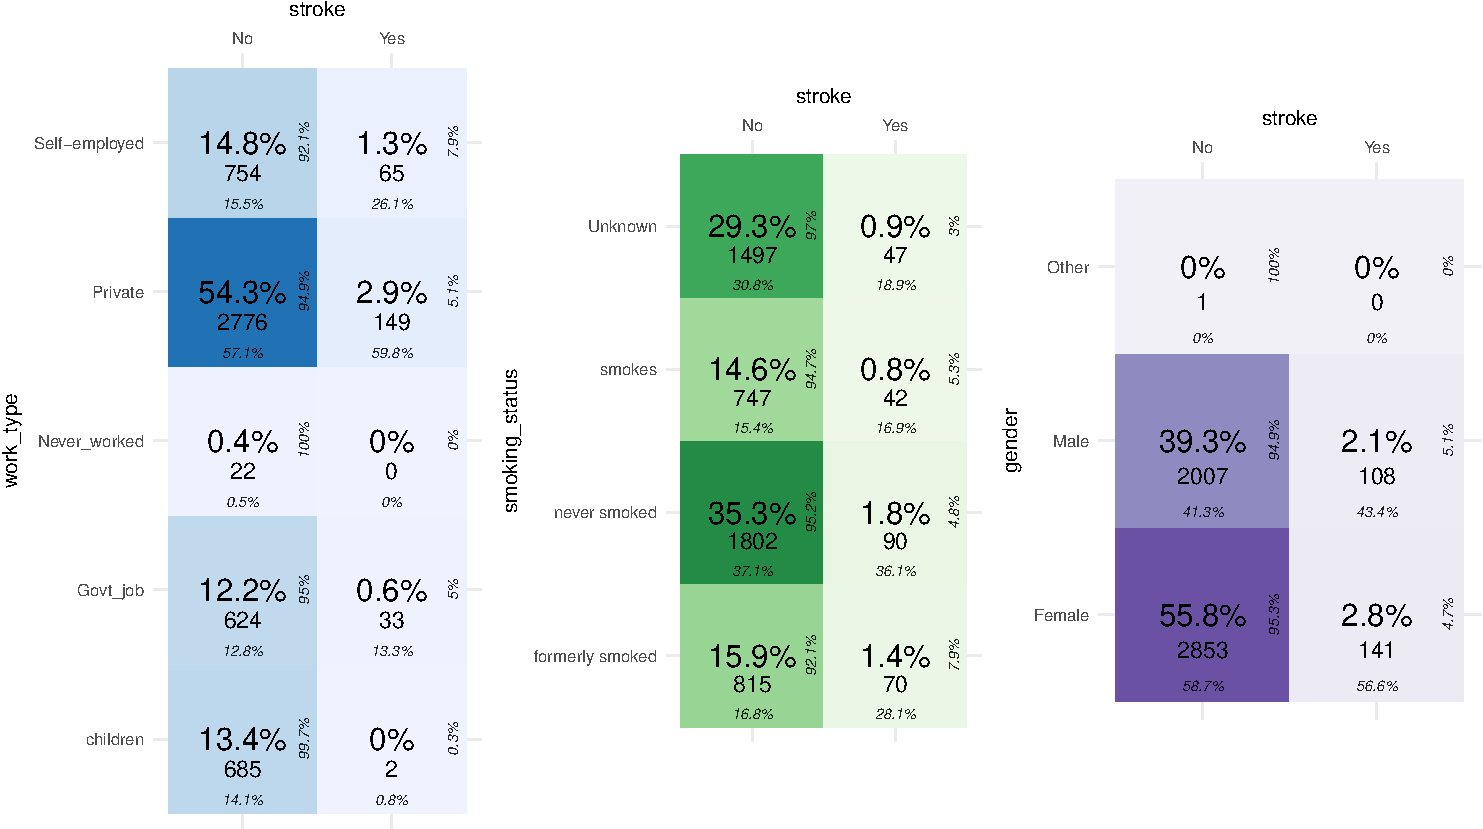
\includegraphics{report2_files/figure-latex/unnamed-chunk-5-1.pdf}

The only interesting information we can retrieve from the plots is that
the youngest (age between 15 and 34) have an \textbf{higher spending
score}, but not other significant information stands out.

\newpage

\section{Dendograms}

Now we start finding subgroups using clustering techniques.

First we used the \textbf{Gower's distance} to build dendrograms with
different methods.\\
This distance can be used to measure how different two records are and
it is always a number between 0 (identical) and 1 (maximally
dissimilar). It is computed as the average of partial dissimilarities
across individuals.

\begin{Shaded}
\begin{Highlighting}[]
\CommentTok{\# Gower distance works for mixed variables}
\NormalTok{malldt.dist}\OtherTok{\textless{}{-}}\FunctionTok{daisy}\NormalTok{(malldt,}\AttributeTok{metric=}\StringTok{"gower"}\NormalTok{)}

\CommentTok{\# Dendrograms}
\NormalTok{malldt.hc.com}\OtherTok{\textless{}{-}}\FunctionTok{hclust}\NormalTok{(malldt.dist,}\AttributeTok{method=}\StringTok{"complete"}\NormalTok{) }
\FunctionTok{plot}\NormalTok{(malldt.hc.com, }\AttributeTok{main=}\StringTok{"Complete Method"}\NormalTok{) }
\FunctionTok{rect.hclust}\NormalTok{(malldt.hc.com,}\AttributeTok{k=}\DecValTok{3}\NormalTok{,}\AttributeTok{border=}\FunctionTok{c}\NormalTok{(}\StringTok{"red"}\NormalTok{,}\StringTok{"green"}\NormalTok{,}\StringTok{"blue"}\NormalTok{)) }
\end{Highlighting}
\end{Shaded}

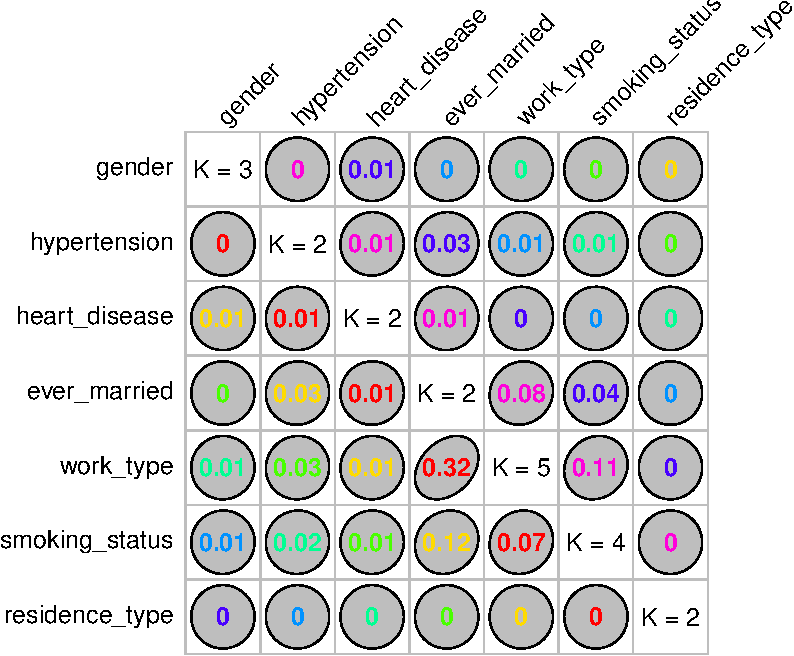
\includegraphics{report2_files/figure-latex/unnamed-chunk-7-1.pdf}

\begin{Shaded}
\begin{Highlighting}[]
\NormalTok{malldt.hc.sin}\OtherTok{\textless{}{-}}\FunctionTok{hclust}\NormalTok{(malldt.dist,}\AttributeTok{method=}\StringTok{"single"}\NormalTok{) }
\FunctionTok{plot}\NormalTok{(malldt.hc.sin, }\AttributeTok{main=}\StringTok{"Single Method"}\NormalTok{) }
\FunctionTok{rect.hclust}\NormalTok{(malldt.hc.sin,}\AttributeTok{k=}\DecValTok{3}\NormalTok{,}\AttributeTok{border=}\FunctionTok{c}\NormalTok{(}\StringTok{"red"}\NormalTok{,}\StringTok{"green"}\NormalTok{,}\StringTok{"blue"}\NormalTok{)) }
\end{Highlighting}
\end{Shaded}

\includegraphics{report2_files/figure-latex/unnamed-chunk-7-2.pdf}

\begin{Shaded}
\begin{Highlighting}[]
\NormalTok{malldt.hc.ave}\OtherTok{\textless{}{-}}\FunctionTok{hclust}\NormalTok{(malldt.dist,}\AttributeTok{method=}\StringTok{"average"}\NormalTok{) }
\FunctionTok{plot}\NormalTok{(malldt.hc.ave, }\AttributeTok{main=}\StringTok{"Average Method"}\NormalTok{) }
\FunctionTok{rect.hclust}\NormalTok{(malldt.hc.ave,}\AttributeTok{k=}\DecValTok{3}\NormalTok{,}\AttributeTok{border=}\FunctionTok{c}\NormalTok{(}\StringTok{"red"}\NormalTok{,}\StringTok{"green"}\NormalTok{,}\StringTok{"blue"}\NormalTok{)) }
\end{Highlighting}
\end{Shaded}

\includegraphics{report2_files/figure-latex/unnamed-chunk-7-3.pdf}

\begin{Shaded}
\begin{Highlighting}[]
\NormalTok{malldt.hc.cen}\OtherTok{\textless{}{-}}\FunctionTok{hclust}\NormalTok{(malldt.dist,}\AttributeTok{method=}\StringTok{"centroid"}\NormalTok{) }
\FunctionTok{plot}\NormalTok{(malldt.hc.cen, }\AttributeTok{main=}\StringTok{"Centroid Method"}\NormalTok{) }
\FunctionTok{rect.hclust}\NormalTok{(malldt.hc.cen,}\AttributeTok{k=}\DecValTok{3}\NormalTok{,}\AttributeTok{border=}\FunctionTok{c}\NormalTok{(}\StringTok{"red"}\NormalTok{,}\StringTok{"green"}\NormalTok{,}\StringTok{"blue"}\NormalTok{)) }
\end{Highlighting}
\end{Shaded}

\includegraphics{report2_files/figure-latex/unnamed-chunk-7-4.pdf}

\begin{Shaded}
\begin{Highlighting}[]
\NormalTok{malldt.hc.ward}\OtherTok{\textless{}{-}}\FunctionTok{hclust}\NormalTok{(malldt.dist,}\AttributeTok{method=}\StringTok{"ward.D2"}\NormalTok{) }
\FunctionTok{plot}\NormalTok{(malldt.hc.ward, }\AttributeTok{main=}\StringTok{"Ward Method"}\NormalTok{) }
\FunctionTok{rect.hclust}\NormalTok{(malldt.hc.ward,}\AttributeTok{k=}\DecValTok{8}\NormalTok{,}\AttributeTok{border=}\FunctionTok{c}\NormalTok{(}\StringTok{"red"}\NormalTok{,}\StringTok{"green"}\NormalTok{,}\StringTok{"blue"}\NormalTok{))}
\end{Highlighting}
\end{Shaded}

\includegraphics{report2_files/figure-latex/unnamed-chunk-7-5.pdf}

\subsection{Ward Method}

The \textbf{Ward Method} is clearly the best one, it detects 8 groups in
our data. Let us count how many observations there are in each group.

\begin{Shaded}
\begin{Highlighting}[]
\CommentTok{\# Allocate obs into 8 groups}
\NormalTok{malldt.groups.ward}\OtherTok{\textless{}{-}}\FunctionTok{cutree}\NormalTok{(malldt.hc.ward,}\AttributeTok{k=}\DecValTok{8}\NormalTok{) }
\NormalTok{malldt.groups.ward}
\end{Highlighting}
\end{Shaded}

\begin{verbatim}
##   [1] 1 1 2 3 2 3 2 3 4 3 4 3 2 3 1 1 2 1 4 3 1 1 2 1 2 1 2 1 2 3 4 3 4 1 2 3 2
##  [38] 3 2 3 5 1 4 3 2 3 5 3 3 3 5 1 3 4 5 4 5 4 3 4 4 1 5 5 4 1 5 5 1 3 4 5 5 5
##  [75] 4 1 5 1 3 5 4 1 4 5 3 4 5 3 5 5 5 1 4 5 3 1 5 3 4 1 3 5 4 1 4 3 5 4 4 4 4
## [112] 3 5 1 3 3 5 5 5 5 1 5 5 6 3 7 8 6 8 6 8 6 3 7 8 7 2 6 8 7 2 6 3 7 8 6 8 7
## [149] 2 6 8 6 2 7 2 7 8 7 8 7 2 7 8 7 8 7 8 7 2 6 8 6 8 6 2 7 8 6 8 6 2 7 8 7 2
## [186] 6 2 6 2 7 2 7 8 7 2 7 2 6 8 6
\end{verbatim}

\begin{Shaded}
\begin{Highlighting}[]
\CommentTok{\# Number of observations in each group}
\FunctionTok{table}\NormalTok{(malldt.groups.ward)}
\end{Highlighting}
\end{Shaded}

\begin{verbatim}
## malldt.groups.ward
##  1  2  3  4  5  6  7  8 
## 25 28 33 25 30 18 21 20
\end{verbatim}

Then for every group we compute the mean value of each variable.

\begin{Shaded}
\begin{Highlighting}[]
\NormalTok{clusterdata.mean}\OtherTok{\textless{}{-}}\ControlFlowTok{function}\NormalTok{(data,groups)\{}
  \FunctionTok{aggregate}\NormalTok{(data,}\FunctionTok{list}\NormalTok{(groups),}\ControlFlowTok{function}\NormalTok{(x)}\FunctionTok{mean}\NormalTok{(}\FunctionTok{as.numeric}\NormalTok{(x)))}
\NormalTok{\}}

\FunctionTok{clusterdata.mean}\NormalTok{(malldt,malldt.groups.ward)}
\end{Highlighting}
\end{Shaded}

\begin{verbatim}
##   Group.1 Gender      Age Annual Income (k$) Spending Score (1-100)
## 1       1      2 25.72000           40.40000               59.00000
## 2       2      1 43.17857           61.78571               21.17857
## 3       3      1 25.45455           43.93939               60.15152
## 4       4      2 58.84000           47.80000               41.00000
## 5       5      1 51.40000           54.96667               49.26667
## 6       6      2 33.27778           87.11111               82.66667
## 7       7      1 32.19048           86.04762               81.66667
## 8       8      2 39.50000           85.15000               14.05000
\end{verbatim}

From this table we can see that there are many groups that are quite
similar to each other, but there are also some interesting differences:

\begin{itemize}
\item \textbf{Gender}: the eight groups are evenly split between ones containing more males and one containing more females. 
\item \textbf{Age}: group 4 and group 5 stand out from the rest, they contain people who tend to be older. Between groups 4 and 5 the only noticeable difference is the **gender**, whereas the other variables are more or less in the same range. \
\item \textbf{Annual income}: the groups could be divided in two. Groups 1 to 5 have annual incomes between 40.000\$ and 60.000\$, then there is quite a big jump in groups 6 to 8, which all have annual incomes above 80.000\$. 
\item \textbf{Spending score}: the spending score varies quite a lot among the groups, even between groups that are similar in other aspects. For example, groups 7 and 8 are quite close in age and annual income, but males appear to have a much higher spending score than females. 

We have obtained a good result, but it can still be improved, since there are clear overlappings between the groups we got.


\section{K-Means algorithm}

In order to refine our grouping, we now apply the K-means algorithm.

First we need to remove the categorical variable **Gender** from the code because
the algorithm only supports numerical variables.


```r
malldtstd<-scale(malldt[,-1]) 
```

\subsection{Finding K}

Then we need to find the right value for k to use in the K-means algorithm.


```r
#set.seed(42)
#k.max<-15 

#wss<-sapply(1:k.max,function(k){kmeans(malldtstd,k,nstart=50,iter.max=15)$tot.withinss})

#plot(1:k.max,wss,type="b",pch=19,xlab="Number of groups",ylab="Within Deviation",col="blue") 
```

Let's try with k=4, k=5 and k=6 and evaluate their performances with the
**silhuotte method**.

\subsection{Silhoutte}

This refers to a method of interpretation and validation of consistency within clusters of data. The technique provides a succinct graphical representation of how well each object has been classified.

The silhouette value is a measure of how similar an object is to its own cluster (cohesion) compared to other clusters (separation). The silhouette ranges from \-1 to +1, where a high value indicates that the object is well matched to its own cluster and poorly matched to neighboring clusters.


```r
kmeans4<-kmeans(malldt[,-1],4)
kmeans5<-kmeans(malldt[,-1],5)
kmeans6<-kmeans(malldt[,-1],6)

# Evaluation of the clustering composition, images will be shown later
#ris4<- eclust(malldt[,-1],"kmeans",k=4)
#ris5<- eclust(malldt[,-1],"kmeans",k=5)
#ris6<- eclust(malldt[,-1],"kmeans",k=6)
```


```r
# Dimensions and average of group's silhouette
avg_s_4 <- fviz_silhouette(ris4) + labs(title= "K = 4",
                                        subtitle= " Avg Silhoutte width: 0.39")
avg_s_5 <- fviz_silhouette(ris5) + labs(title= "K = 5",
                                        subtitle= " Avg Silhoutte width: 0.38")
avg_s_6 <- fviz_silhouette(ris6)+ labs(title= "K = 6",
                                        subtitle= " Avg Silhoutte width: 0.34")
```


![](report2_files/figure-latex/unnamed-chunk-15-1.pdf)<!-- --> 


From the plots on the left we can see whether the groups are well defined or they overlap.
It is clear that the higher is the value of k, the bigger are the problems of overlapping.

Moreover, as we can see from the plots on the right, k=4 has also the best average silhouette value (0.39). From these plots it is also evident that k=4 has no observation with a negative silhouette value.

We decided to check this last point, searching for every exact observations with a negative silhouette value.



```r
# Silhouette measure of each observation
sil4<-ris4$silinfo$widths 
sil5<-ris5$silinfo$widths
sil6<-ris6$silinfo$widths

# Position of observation of silhouette < 0
neg_sil_index4<-which(sil4[,'sil_width']<0)
neg_sil_index5<-which(sil5[,'sil_width']<0)
neg_sil_index6<-which(sil6[,'sil_width']<0)

# Observations with silhouette < 0
sil4[neg_sil_index4,]
```

```
## [1] cluster   neighbor  sil_width
## <0 rows> (or 0-length row.names)
```

```r
sil5[neg_sil_index5,]
```

```
##     cluster neighbor    sil_width
## 5         1        3 -0.002970177
## 81        1        5 -0.010702602
## 51        1        5 -0.015719656
## 64        1        5 -0.042706823
## 72        1        5 -0.125272449
## 80        1        5 -0.185484474
## 147       2        5 -0.004406397
```

```r
sil6[neg_sil_index6,]
```

```
##     cluster neighbor    sil_width
## 173       1        2 -0.032252777
## 115       6        1 -0.004885339
## 114       6        1 -0.016919517
## 122       6        2 -0.018699176
## 53        6        3 -0.019420998
## 85        6        3 -0.039947417
## 92        6        1 -0.040483768
## 106       6        1 -0.048138547
## 101       6        1 -0.051225653
## 5         6        3 -0.058976374
```

This again confirms that with k=4 we obtain zero observations with negative silhouette value, whereas with k=5 and k=6 we have respectively 7 and 10 observation of this kind.

Now that we have found the best value to use for 4, we plot another dendrogram using the Ward Method but splitting it in just 4 gorups.


```r
malldt.hc.ward.1<-hclust(malldt.dist,method="ward.D2") 
plot(malldt.hc.ward.1, main="Ward Method") 
rect.hclust(malldt.hc.ward.1,k=4,border=c("red","green","blue"))
```

![](report2_files/figure-latex/unnamed-chunk-17-1.pdf)<!-- --> 

Now let's see the means of the variables in the new groups to try and identify the characteristics that define the groups.


```r
# Allocate obs into 4 groups
malldt.groups.ward.1<-cutree(malldt.hc.ward.1 ,k=4) 
malldt.groups.ward.1
```

```
##   [1] 1 1 2 3 2 3 2 3 4 3 4 3 2 3 1 1 2 1 4 3 1 1 2 1 2 1 2 1 2 3 4 3 4 1 2 3 2
##  [38] 3 2 3 2 1 4 3 2 3 2 3 3 3 2 1 3 4 2 4 2 4 3 4 4 1 2 2 4 1 2 2 1 3 4 2 2 2
##  [75] 4 1 2 1 3 2 4 1 4 2 3 4 2 3 2 2 2 1 4 2 3 1 2 3 4 1 3 2 4 1 4 3 2 4 4 4 4
## [112] 3 2 1 3 3 2 2 2 2 1 2 2 1 3 3 4 1 4 1 4 1 3 3 4 3 2 1 4 3 2 1 3 3 4 1 4 3
## [149] 2 1 4 1 2 3 2 3 4 3 4 3 2 3 4 3 4 3 4 3 2 1 4 1 4 1 2 3 4 1 4 1 2 3 4 3 2
## [186] 1 2 1 2 3 2 3 4 3 2 3 2 1 4 1
```

```r
# Number of observations in each group
table(malldt.groups.ward.1)
```

```
## malldt.groups.ward.1
##  1  2  3  4 
## 43 58 54 45
```


```r
clusterdata.mean(malldt,malldt.groups.ward.1)
```

```
##   Group.1 Gender      Age Annual Income (k$) Spending Score (1-100)
## 1       1      2 28.88372           59.95349               68.90698
## 2       2      1 47.43103           58.25862               35.70690
## 3       3      1 28.07407           60.31481               68.51852
## 4       4      2 50.24444           64.40000               29.02222
```

Now that the data is divided in 4 groups, some other observations can be done:
\begin{itemize}
\item \textbf{Gender}: the groups are still evenly split between females and males.
\item \textbf{Age}: there is also a pretty even split in age. Two groups contain people that are around 30 years old on average and two groups are composed of people who are around 50 years old on average.
\item \textbf{Annual income}: now the annual income is pretty even among the four groups, at around 60.000\$. 
\item \textbf{Spending Score}: the spending scores can again be split in two. Younger people have a higher spending score than older people.
\end{itemize}

At this point, looking at these results, we could name and describe the
four groups in the following way:

\begin{itemize}
\item \textbf{Group 1}: \textbf{Young Females}, average annual income and high spending score.
\item \textbf{Group 2}: \textbf{Old Males}, average annual income and low spending score.
\item \textbf{Group 3}: \textbf{Young Males}, average annual income and high spending score.
\item \textbf{Group 4}: \textbf{Old Females}, average annual income and low spending score.
\end{itemize}

What emerged from this analysis is that for the same average annual
income, younger people have a tendency to spend more than older people
at a mall. Moreover, these spending habits seem not to be influenced by
the gender of a given individual but solely by the age.

\end{document}
